% EE582 HW02 Report
% Author: Aryan  
% Date: October 2025

\documentclass[12pt]{article}
\usepackage{amsmath, amssymb, graphicx, float, hyperref}
\usepackage{cleveref}
\usepackage[margin=1in]{geometry}
\usepackage{enumitem}
\usepackage{siunitx}
\usepackage{tikz}
\usepackage{circuitikz}
\usepackage{mathtools}
\usepackage{xcolor}
\usepackage{array}
\usepackage{colortbl}
\usepackage{multirow}
\usepackage{tcolorbox}
\usepackage{fancyhdr}
\usepackage{booktabs}

% Setup page headers
\setlength{\headheight}{14.49998pt}
\pagestyle{fancy}
\fancyhf{}
\fancyhead[R]{\rightmark}
\fancyfoot[C]{\thepage}
\renewcommand{\headrulewidth}{0.4pt}
\renewcommand{\sectionmark}[1]{\markboth{#1}{#1}}
\renewcommand{\subsectionmark}[1]{\markright{#1}}

% Custom section numbering: subsections get A.1.1, A.1.2, etc.
\setcounter{secnumdepth}{3}  % Enable numbering for subsections
\setcounter{tocdepth}{1}  % Only show sections in TOC, not subsections
\newcommand{\sectionprefix}{}  % Define command to hold section prefix
\renewcommand{\thesubsection}{\sectionprefix.\arabic{subsection}}

\title{Fall 2025 EE582 Homework 02 Report \\ Nodal-Analysis-based Modeling of Electric Circuits}
\author{Aryan Ritwajeet Jha}
\date{Due: Tuesday, October 7, 2025}

\begin{document}
\maketitle

\tableofcontents

% Section A Questions
\clearpage
\section*{Section A (Numerical Oscillations of Discretization Rules)}
\addcontentsline{toc}{section}{Section A (Numerical Oscillations of Discretization Rules)}

One way to analyze the properties of various discretization methods (e.g., in terms of their numerical oscillations) is to solve a lossless first-order system (e.g., inductance or capacitance) when the state variable of the component is suddenly changed. The circuit on the right considers a case where a dc voltage is suddenly applied to a capacitor. Because the source voltage is applied like a step function, we know that the current of the capacitor should look like an impulse, analytically. Let us assume that in the simulations all the variables are zero at $t=0$ and the voltage source takes its value at $t=\Delta t$.

\begin{figure}[h!]
    \centering
    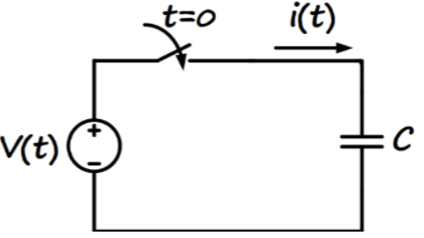
\includegraphics[width=0.4\textwidth]{figures/figure-A-circuit.png}
    \caption{Simple capacitor circuit with DC voltage source}
    \label{fig:a01_circuit}
\end{figure}

1) Determine the step-by-step solution for the current in the capacitor (in terms of capacitance $C$, time-step size $\Delta t$, and source voltage) using the following discretization rules: a) Forward Euler, b) Backward Euler, c) Trapezoidal.

\vspace{1em}
% Your solution here

\clearpage
\renewcommand{\sectionprefix}{A.2}  % Set prefix for this question
\setcounter{subsection}{0}  % Reset subsection counter
\section*{Section A: Question 2}
\addcontentsline{toc}{section}{Section A: Question 2}

Comment on how the simulation time-step size impacts the numerical solution, and which method is preferred in this case.

\noindent\rule{\textwidth}{0.4pt}

\subsection{Simulation Parameters}

I implemented all three discretization methods in MATLAB with the following circuit parameters: $V_{DC} = 10$ V, $V_0 = 0$ V, $C = 1\,\mu$F, and $h = 100\,\mu$s. I also simulated the Trapezoidal method in PSCAD with chatter attenuation disabled to allow direct comparison with the analytical solution.

\subsection{Method Comparison and Selection}

\subsubsection*{Forward Euler: Rejected}

The Forward Euler method exhibits catastrophic numerical instability, as demonstrated in \Cref{fig:a02_fe_detail}. The current diverges exponentially with an amplification factor of $(R_c/R_{\epsilon})^n \approx 10^{3n}$ at step $n$ (Note that I've taken $R_\epsilon = R_c/1000$), reaching magnitudes exceeding $10^{17}$ A within microseconds. This non-physical behavior renders the method completely unsuitable for this circuit. Due to its extreme divergence, Forward Euler is shown separately and not included in the comparison plot with the other two methods.

\begin{figure}[h!]
    \centering
    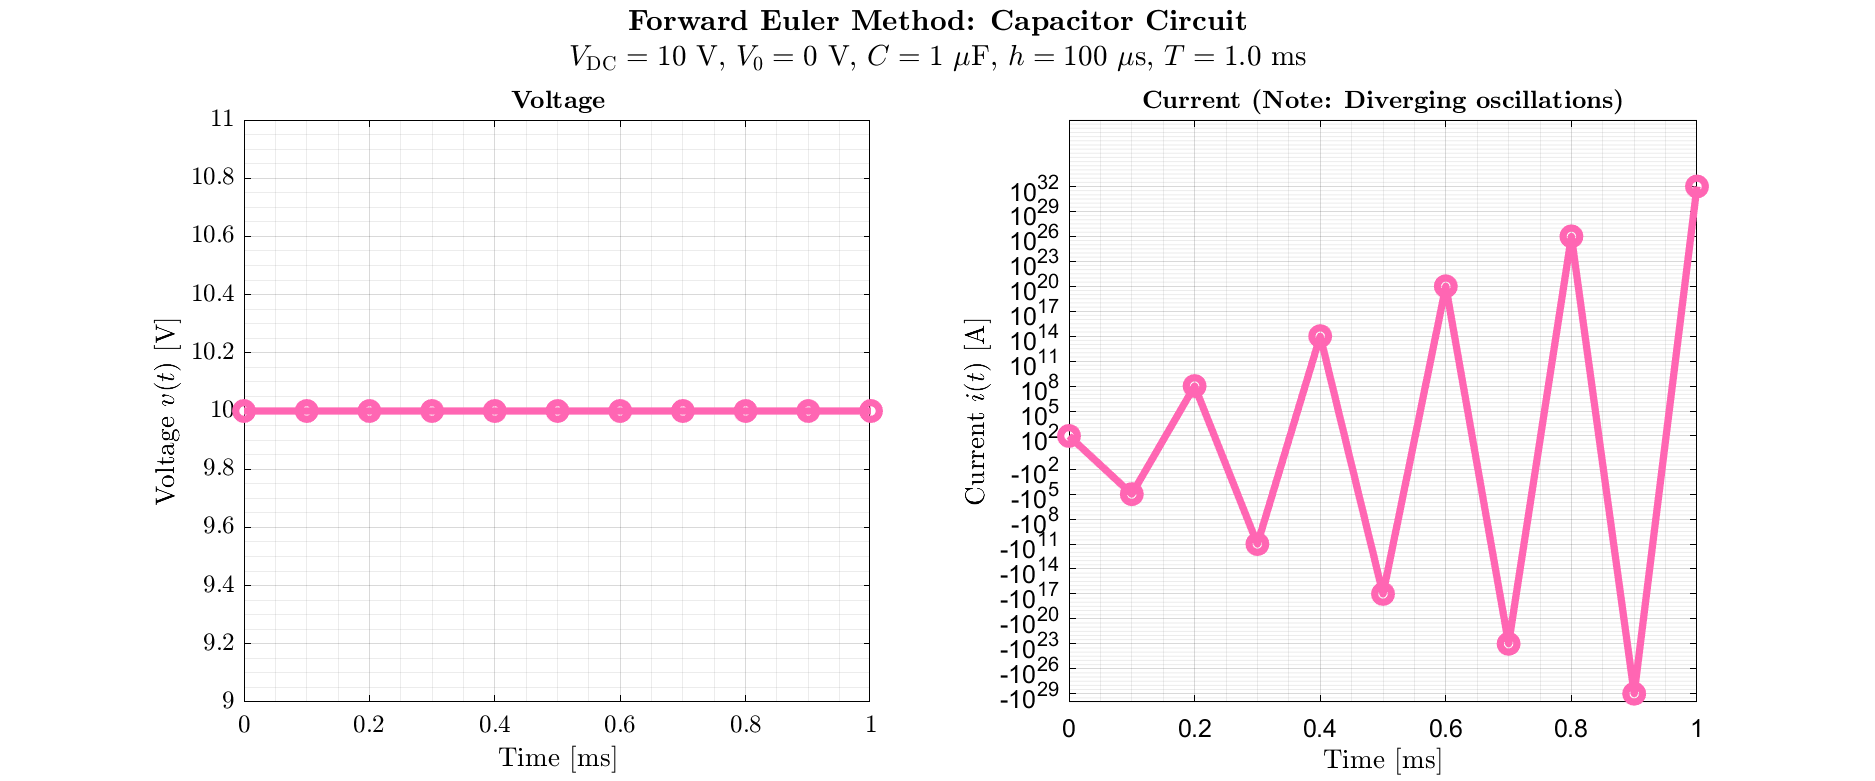
\includegraphics[width=0.85\textwidth]{figures/hw02_qA_forward-euler-method.png}
    \caption{Forward Euler method showing exponential divergence in current magnitude (symmetric logarithmic scale). The oscillations grow with successive powers of $(R_c/R_\epsilon)$, demonstrating fundamental numerical instability.}
    \label{fig:a02_fe_detail}
\end{figure}

\subsubsection*{Backward Euler vs. Trapezoidal}

\Cref{fig:a02_comparison} compares the Backward Euler and Trapezoidal methods against the PSCAD reference solution. 

\begin{figure}[h!]
    \centering
    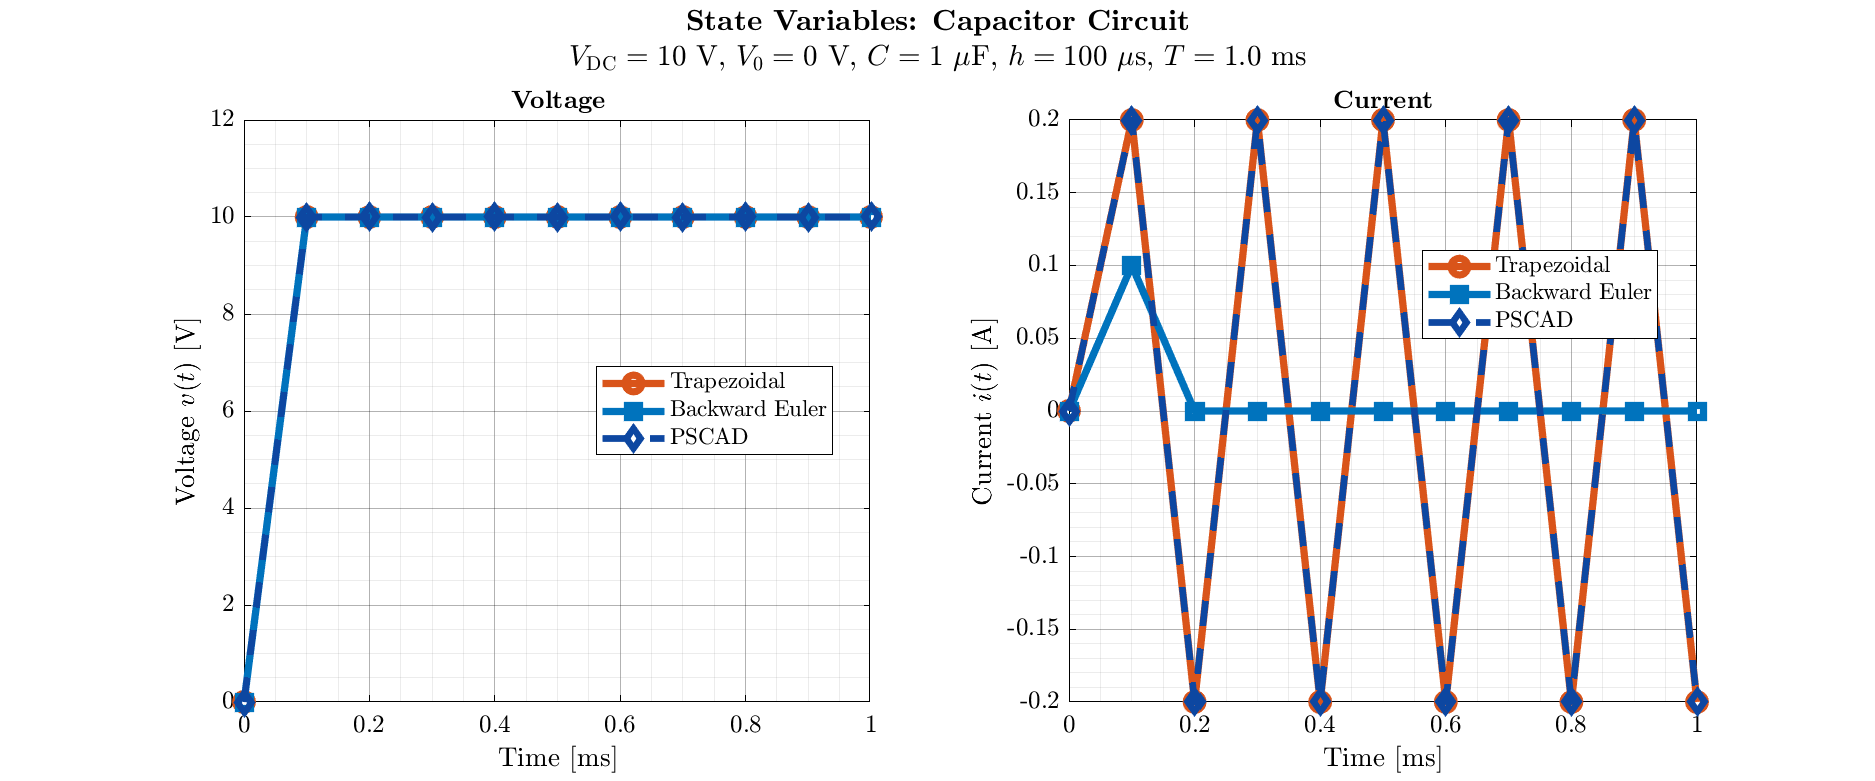
\includegraphics[width=0.85\textwidth]{figures/hw02_qA_state-variable-trajectory-comparison.png}
    \caption{Comparison of Backward Euler, Trapezoidal, and PSCAD solutions. BE provides maximum damping (minimizing current oscillations), while Trapezoidal matches PSCAD exactly and exhibits numerical chatter characteristic of lossless circuit discretization.}
    \label{fig:a02_comparison}
\end{figure}

Key observations:

\begin{itemize}
    \item \textbf{Backward Euler}: Provides maximum numerical damping, driving $i(t) \to 0$ after the initial transient. This represents the \textit{closest approach to the true steady-state solution} (zero current after capacitor charges), effectively suppressing the numerical oscillations entirely.
    
    \item \textbf{Trapezoidal}: Exhibits sustained bounded oscillations (``chatter'') due to its energy-preserving nature. My MATLAB implementation and PSCAD solution (with chatter attenuation disabled) are \textit{identical}, confirming correct implementation. The chatter is a numerical artifact of discretizing a lossless system.
    
    \item \textbf{PSCAD with chatter enabled}: When chatter attenuation is enabled in PSCAD, the solution approaches the BE behavior, demonstrating that PSCAD internally applies damping to suppress numerical oscillations.
\end{itemize}

\subsection{Impact of Step Size}

\begin{itemize}
    \item \textbf{Smaller $h$}: Reduces $R_C = h/(2C)$ for Trapezoidal, increasing chatter magnitude but maintaining stability. For BE, reduces artificial damping.
    \item \textbf{Larger $h$}: Increases numerical damping in BE (faster convergence to zero) and reduces chatter amplitude in Trapezoidal. Both remain stable.
    \item \textbf{Forward Euler}: Unstable for any step size due to the amplification factor exceeding unity.
\end{itemize}

\subsection{Preferred Method}

\textbf{Backward Euler} is preferred for this specific problem because it most closely represents the true steady-state behavior (zero current after capacitor fully charges), effectively eliminating the non-physical chatter artifacts. While Trapezoidal offers higher accuracy for transient analysis and matches PSCAD's unattenuated solution, the BE method's numerical damping produces the most physically meaningful result for a lossless capacitor reaching steady state.


% Section B Questions  
\clearpage
\section*{Section B: Question 1}
\addcontentsline{toc}{section}{Section B: Question 1}

The parameters of the circuit below are: $R=10\Omega, L=20mH, e(t)=10V dc$, and the switch is closed at $t=0$. The circuit is to be solved from $t=0$ to $t=10ms$ using:

\begin{enumerate}[label=\alph*)]
  \item PSCAD software,
  \item your own MATLAB code based on the nodal analysis method.
\end{enumerate}

\vspace{1em}
% Your solution here

\clearpage
\renewcommand{\sectionprefix}{B.2}  % Set prefix for this question
\setcounter{subsection}{0}  % Reset subsection counter
\section*{Section B : Question 2}
\addcontentsline{toc}{section}{Section B: Question 2}

2) Discretize the circuit and write a MATLAB code to solve the circuit step-by-step using the two discretization rules: a) Backward Euler, b) Trapezoidal, each with time-step sizes $\Delta t = 0.1\text{ms}$ and $\Delta t = 0.8\text{ms}$.

\noindent\rule{\textwidth}{0.4pt}

% Your solution here

\vspace{1em}
\noindent\rule{\textwidth}{0.4pt}
\clearpage
\section*{Section B : Question 3}
\addcontentsline{toc}{section}{Section B : Question 3}

3) Show the results for $i(t)$ obtained in the six cases (PSCAD, your Backward Euler code, and your Trapezoidal code; each with two different step sizes) superimposed in a (big enough) Plot. Show the same for $v_L(t)$ in a separate plot. Comment on the accuracy of the methods, impact of the time-step size, and how the PSCAD results compare with your Trapezoidal code.

\vspace{1em}

% Your solution here

% Section C Questions
\clearpage
\section*{Section C (Circuit Interruption): Question 1}
\addcontentsline{toc}{section}{Section C (Circuit Interruption): Question 1}

The case below (figure on the left) represents a typical short-circuit fault in transmission lines and the breaker operation for line interruption. The equivalent circuit is shown in the figure on the right.

\begin{figure}[h!]
    \centering
    \begin{minipage}{0.45\textwidth}
        \centering
        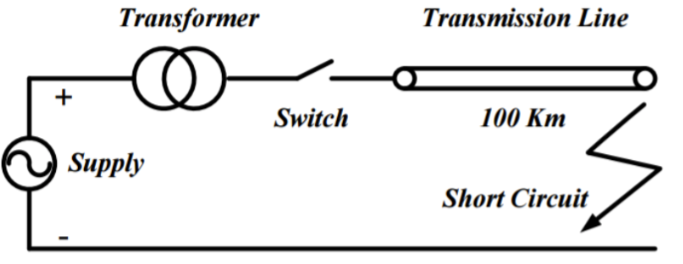
\includegraphics[width=\textwidth]{figures/figure-C-circuit-left.png}
        \caption{Transmission line with short-circuit fault}
        \label{fig:c01_circuit_left}
    \end{minipage}
    \hfill
    \begin{minipage}{0.45\textwidth}
        \centering
        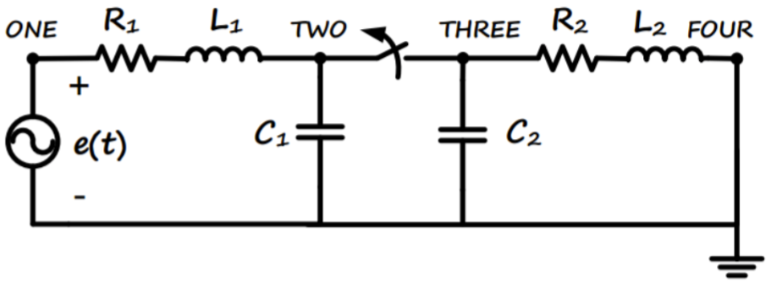
\includegraphics[width=\textwidth]{figures/figure-C-circuit-right.png}
        \caption{Equivalent circuit representation}
        \label{fig:c01_circuit_right}
    \end{minipage}
\end{figure}

On the left-hand side of the switch/breaker, we have the source voltage and a resistance and inductance representing the supply system combined with the transformer. The capacitor to the left of the breaker represents the combined substation capacitance due to the substation busbars. On the right-hand side of the breaker, we have the transmission line parameters: resistance, inductance, and capacitance represented as simple lumped parameters, where the right side is short-circuited due to the fault, assuming that the fault has already been applied. We have assumed a single-phase circuit here for simplicity. The parameters of the circuit below are: $e(t) = 230\times\cos(\omega t)$ kV, $\omega=377$ rad/s, $R_1=3\Omega$, $L_1=350$ mH, $R_2=50\Omega$, $L_2=100$ mH, $C_1=10$ nF, $C_2=600$ nF. Assume that the system is operating with zero initial conditions and the breaker is initially closed. At $t=8$ ms, the breaker is commanded to open the line, but it will not actually open until the current passes through zero. The study period is from $t=0$ to $t=20$ ms.

1) Choose an appropriate simulation time-step size $\Delta t$ (assuming the Trapezoidal integration rule) according to the time constants in the circuit. For this, evaluate the approximate resonant frequencies analytically before and after the breaker operation.

\noindent\rule{\textwidth}{0.4pt}

% Your solution here
\clearpage
\renewcommand{\sectionprefix}{C.2}  % Set prefix for this question
\setcounter{subsection}{0}  % Reset subsection counter
\section*{Section C: Question 2}
\markboth{Section C: Question 2}{Section C: Question 2}
\addcontentsline{toc}{section}{Section C: Question 2}
\renewcommand{\subsectionmark}[1]{}

\textbf{Problem Statement:} The case below (figure on the left) represents a typical short-circuit fault in transmission lines and the breaker operation for line interruption. The equivalent circuit is shown in the figure on the right.

\begin{figure}[h!]
    \centering
    \begin{minipage}{0.45\textwidth}
        \centering
        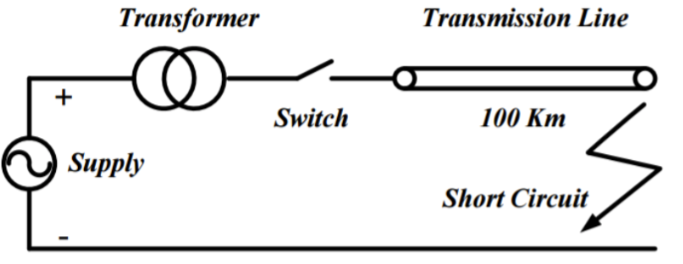
\includegraphics[width=\textwidth]{figures/figure-C-circuit-left.png}
        \caption{Transmission line with short-circuit fault}
        \label{fig:c02_circuit_left}
    \end{minipage}
    \hfill
    \begin{minipage}{0.45\textwidth}
        \centering
        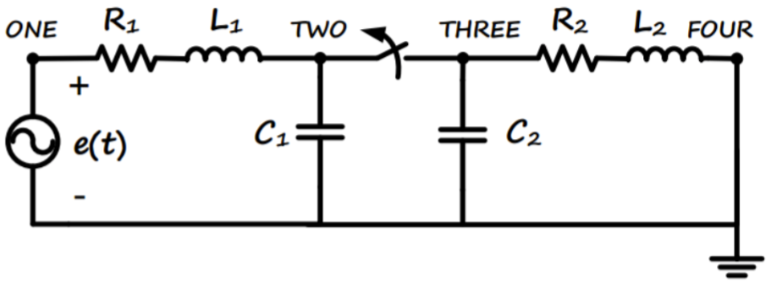
\includegraphics[width=\textwidth]{figures/figure-C-circuit-right.png}
        \caption{Equivalent circuit representation}
        \label{fig:c02_circuit_right}
    \end{minipage}
\end{figure}

On the left-hand side of the switch/breaker, we have the source voltage and a resistance and inductance representing the supply system combined with the transformer. The capacitor to the left of the breaker represents the combined substation capacitance due to the substation busbars. On the right-hand side of the breaker, we have the transmission line parameters: resistance, inductance, and capacitance represented as simple lumped parameters, where the right side is short-circuited due to the fault, assuming that the fault has already been applied. We have assumed a single-phase circuit here for simplicity. The parameters of the circuit below are: $e(t) = 230\times\cos(\omega t)$ kV, $\omega=377$ rad/s, $R_1=3\Omega$, $L_1=350$ mH, $R_2=50\Omega$, $L_2=100$ mH, $C_1=10$ nF, $C_2=600$ nF. Assume that the system is operating with zero initial conditions and the breaker is initially closed. At $t=8$ ms, the breaker is commanded to open the line, but it will not actually open until the current passes through zero. The study period is from $t=0$ to $t=20$ ms.

2) Write your own MATLAB code to solve the system and also obtain the solution using PSCAD.

\noindent\rule{\textwidth}{0.4pt}

\vspace{1em}

\textbf{Solution:}

\subsection{Nodal Analysis and Equivalent Circuit Diagrams}

To implement the MATLAB solution, we first need to establish the equivalent circuit diagrams for the nodal analysis method. The circuit behavior changes based on the breaker state.

\begin{figure}[H]
    \centering
    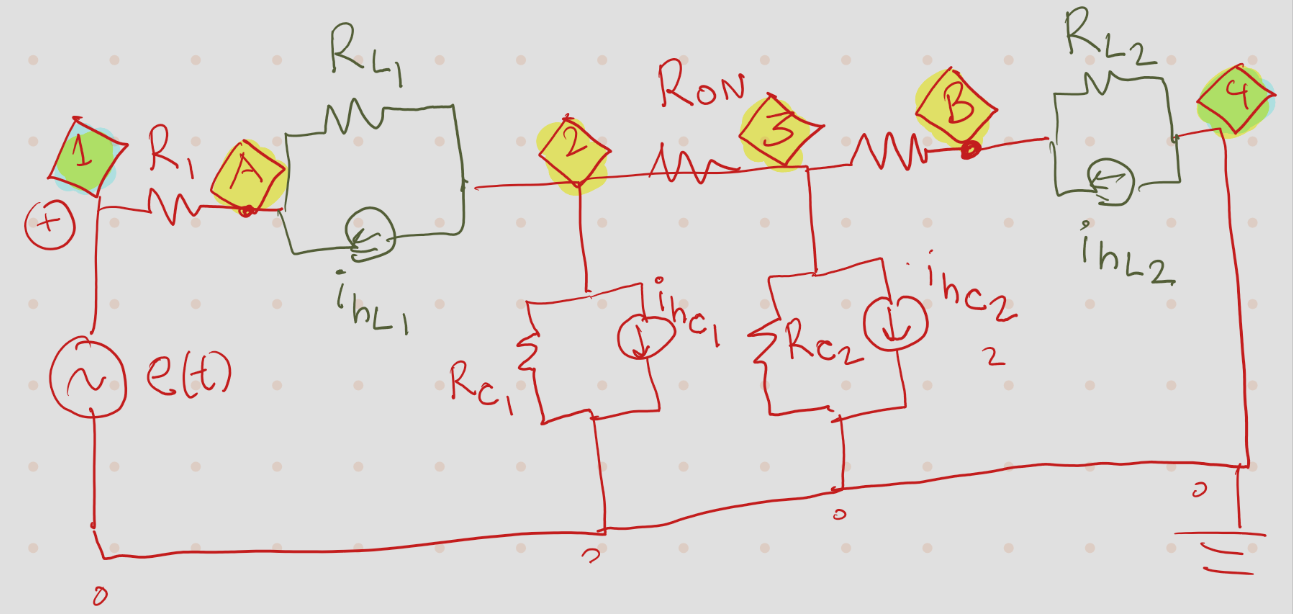
\includegraphics[width=0.85\textwidth]{figures/qC-nodal-ckt-equiv-diag-swt-closed-handdrawn.png}
    \caption{Equivalent circuit diagram for nodal analysis when switch is closed (breaker closed state). Note that the nodes highlighted in green are connected to voltage sources or ground, while those in yellow are unknowns. This configuration will be used to construct the conductance matrix $\mathbf{G}$ for $t < t_{\text{open, actual}}$.}
    \label{fig:c02_nodal_closed}
\end{figure}

\begin{figure}[H]
    \centering
    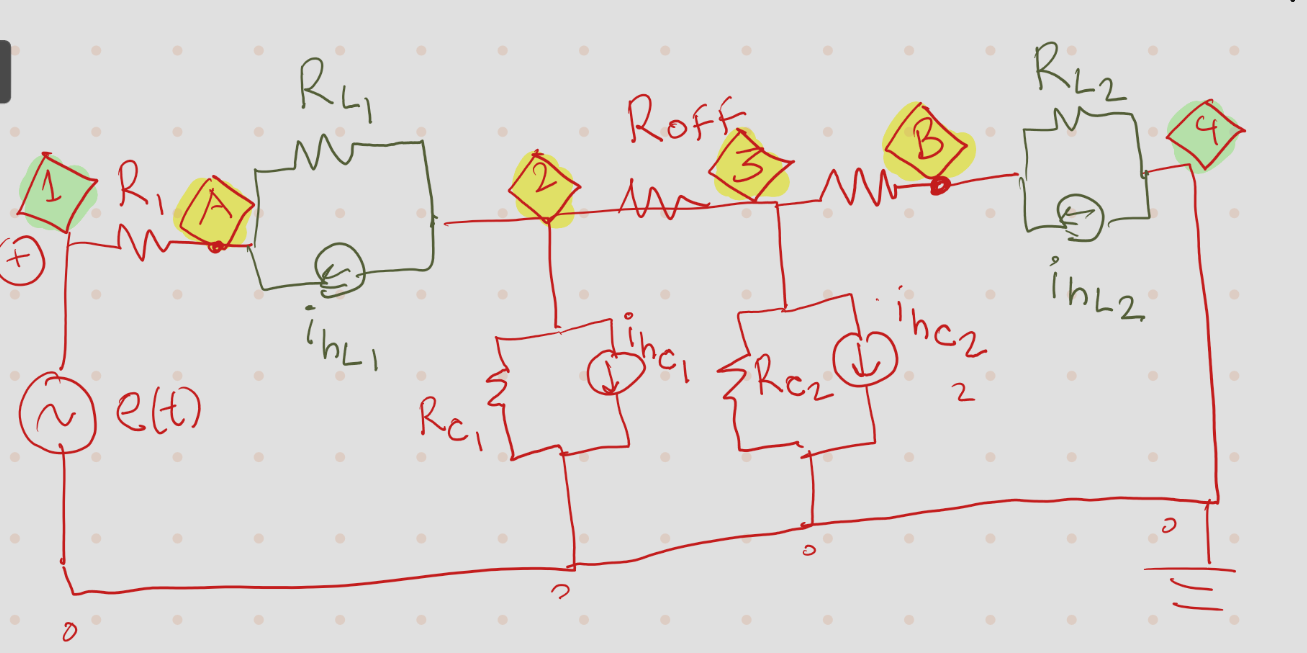
\includegraphics[width=0.85\textwidth]{figures/qC-nodal-ckt-equiv-diag-swt-opened-handdrawn.png}
    \caption{Equivalent circuit diagram for nodal analysis when switch is opened (breaker open state). Note that the nodes highlighted in green are connected to voltage sources or ground, while those in yellow are unknowns.This configuration will be used to construct the conductance matrix $\mathbf{G}$ for $t \geq t_{\text{open, actual}}$.}
    \label{fig:c02_nodal_open}
\end{figure}

These equivalent circuit diagrams show the companion models for the inductors and capacitors, which will be referenced when building the conductance matrices $\mathbf{G}$ for the nodal analysis formulation.

% Your solution here

\vspace{1em}
\noindent\rule{\textwidth}{0.4pt}
\clearpage
\section*{Section C : Question 3}
\addcontentsline{toc}{section}{Section C : Question 3}

3) Show the results for voltages at nodes $Two$ and $Three$ and the fault current (i.e., from node $Four$ to $ground$) in three separate (big enough) plots. In each plot, superimpose the results from your code and also from PSCAD, both obtained using the same simulation time-step size obtained in part 1) for comparison. Comment on the accuracy of your results compared to those of PSCAD.

\vspace{1em}

% Your solution here

\clearpage
\appendix
\renewcommand{\thesection}{\Roman{section}}

% Add appendix reference
\clearpage
\section{Derivation of Trapezoidal Discretization Equations} \label{sec:appendix_derivation}
The governing equation for a capacitor is given by:
\begin{equation}
    i(t) = C \frac{dv(t)}{dt}
\end{equation}
Using the trapezoidal rule, the discretized forms for the voltage $v(t)$ and current $i(t)$ are derived as follows:

\paragraph{Core Relation:}
\begin{equation}
    v(t) - v(t - \Delta t) = \frac{\Delta t}{2C} \left[ i(t) + i(t - \Delta t) \right]
\end{equation}
Define the equivalent resistance $R_C$ and history terms:
\begin{equation}
    R_C = \frac{\Delta t}{2C}
\end{equation}

\subsubsection*{1) Thevenin (Series) Companion}
Rewriting the core relation:
\begin{equation}
    v(t) = \left[ v(t - \Delta t) + R_C i(t - \Delta t) \right] + R_C i(t)
\end{equation}
Here, the capacitor at step $t$ is a voltage source $e_h$ in series with $R_C$:
\begin{equation}
    v(t) = e_h + R_C i(t)
\end{equation}
with the history voltage:
\begin{equation}
    e_h = v(t - \Delta t) + R_C i(t - \Delta t)
\end{equation}

\subsubsection*{2) Norton (Parallel) Companion}
From the core relation:
\begin{equation}
    \frac{v(t) - v(t - \Delta t)}{R_C} = i(t) + i(t - \Delta t)
\end{equation}
Rewriting:
\begin{equation}
    i(t) = \frac{v(t)}{R_C} - \left[ \frac{v(t - \Delta t)}{R_C} - i(t - \Delta t) \right]
\end{equation}
Here, the capacitor at step $t$ is a current source $i_h$ in parallel with conductance $1/R_C$:
\begin{equation}
    i(t) = \frac{v(t)}{R_C} - i_h
\end{equation}
with the history current:
\begin{equation}
    i_h = \frac{v(t - \Delta t)}{R_C} - i(t - \Delta t)
\end{equation}
\end{document}
